\documentclass[]{article}
\usepackage{lmodern}
\usepackage{amssymb,amsmath}
\usepackage{ifxetex,ifluatex}
\usepackage{fixltx2e} % provides \textsubscript
\ifnum 0\ifxetex 1\fi\ifluatex 1\fi=0 % if pdftex
  \usepackage[T1]{fontenc}
  \usepackage[utf8]{inputenc}
\else % if luatex or xelatex
  \ifxetex
    \usepackage{mathspec}
  \else
    \usepackage{fontspec}
  \fi
  \defaultfontfeatures{Ligatures=TeX,Scale=MatchLowercase}
\fi
% use upquote if available, for straight quotes in verbatim environments
\IfFileExists{upquote.sty}{\usepackage{upquote}}{}
% use microtype if available
\IfFileExists{microtype.sty}{%
\usepackage{microtype}
\UseMicrotypeSet[protrusion]{basicmath} % disable protrusion for tt fonts
}{}
\usepackage[margin=1in]{geometry}
\usepackage{hyperref}
\hypersetup{unicode=true,
            pdftitle={data\_exploration},
            pdfauthor={Nikki Shintaku},
            pdfborder={0 0 0},
            breaklinks=true}
\urlstyle{same}  % don't use monospace font for urls
\usepackage{color}
\usepackage{fancyvrb}
\newcommand{\VerbBar}{|}
\newcommand{\VERB}{\Verb[commandchars=\\\{\}]}
\DefineVerbatimEnvironment{Highlighting}{Verbatim}{commandchars=\\\{\}}
% Add ',fontsize=\small' for more characters per line
\usepackage{framed}
\definecolor{shadecolor}{RGB}{248,248,248}
\newenvironment{Shaded}{\begin{snugshade}}{\end{snugshade}}
\newcommand{\AlertTok}[1]{\textcolor[rgb]{0.94,0.16,0.16}{#1}}
\newcommand{\AnnotationTok}[1]{\textcolor[rgb]{0.56,0.35,0.01}{\textbf{\textit{#1}}}}
\newcommand{\AttributeTok}[1]{\textcolor[rgb]{0.77,0.63,0.00}{#1}}
\newcommand{\BaseNTok}[1]{\textcolor[rgb]{0.00,0.00,0.81}{#1}}
\newcommand{\BuiltInTok}[1]{#1}
\newcommand{\CharTok}[1]{\textcolor[rgb]{0.31,0.60,0.02}{#1}}
\newcommand{\CommentTok}[1]{\textcolor[rgb]{0.56,0.35,0.01}{\textit{#1}}}
\newcommand{\CommentVarTok}[1]{\textcolor[rgb]{0.56,0.35,0.01}{\textbf{\textit{#1}}}}
\newcommand{\ConstantTok}[1]{\textcolor[rgb]{0.00,0.00,0.00}{#1}}
\newcommand{\ControlFlowTok}[1]{\textcolor[rgb]{0.13,0.29,0.53}{\textbf{#1}}}
\newcommand{\DataTypeTok}[1]{\textcolor[rgb]{0.13,0.29,0.53}{#1}}
\newcommand{\DecValTok}[1]{\textcolor[rgb]{0.00,0.00,0.81}{#1}}
\newcommand{\DocumentationTok}[1]{\textcolor[rgb]{0.56,0.35,0.01}{\textbf{\textit{#1}}}}
\newcommand{\ErrorTok}[1]{\textcolor[rgb]{0.64,0.00,0.00}{\textbf{#1}}}
\newcommand{\ExtensionTok}[1]{#1}
\newcommand{\FloatTok}[1]{\textcolor[rgb]{0.00,0.00,0.81}{#1}}
\newcommand{\FunctionTok}[1]{\textcolor[rgb]{0.00,0.00,0.00}{#1}}
\newcommand{\ImportTok}[1]{#1}
\newcommand{\InformationTok}[1]{\textcolor[rgb]{0.56,0.35,0.01}{\textbf{\textit{#1}}}}
\newcommand{\KeywordTok}[1]{\textcolor[rgb]{0.13,0.29,0.53}{\textbf{#1}}}
\newcommand{\NormalTok}[1]{#1}
\newcommand{\OperatorTok}[1]{\textcolor[rgb]{0.81,0.36,0.00}{\textbf{#1}}}
\newcommand{\OtherTok}[1]{\textcolor[rgb]{0.56,0.35,0.01}{#1}}
\newcommand{\PreprocessorTok}[1]{\textcolor[rgb]{0.56,0.35,0.01}{\textit{#1}}}
\newcommand{\RegionMarkerTok}[1]{#1}
\newcommand{\SpecialCharTok}[1]{\textcolor[rgb]{0.00,0.00,0.00}{#1}}
\newcommand{\SpecialStringTok}[1]{\textcolor[rgb]{0.31,0.60,0.02}{#1}}
\newcommand{\StringTok}[1]{\textcolor[rgb]{0.31,0.60,0.02}{#1}}
\newcommand{\VariableTok}[1]{\textcolor[rgb]{0.00,0.00,0.00}{#1}}
\newcommand{\VerbatimStringTok}[1]{\textcolor[rgb]{0.31,0.60,0.02}{#1}}
\newcommand{\WarningTok}[1]{\textcolor[rgb]{0.56,0.35,0.01}{\textbf{\textit{#1}}}}
\usepackage{longtable,booktabs}
\usepackage{graphicx,grffile}
\makeatletter
\def\maxwidth{\ifdim\Gin@nat@width>\linewidth\linewidth\else\Gin@nat@width\fi}
\def\maxheight{\ifdim\Gin@nat@height>\textheight\textheight\else\Gin@nat@height\fi}
\makeatother
% Scale images if necessary, so that they will not overflow the page
% margins by default, and it is still possible to overwrite the defaults
% using explicit options in \includegraphics[width, height, ...]{}
\setkeys{Gin}{width=\maxwidth,height=\maxheight,keepaspectratio}
\IfFileExists{parskip.sty}{%
\usepackage{parskip}
}{% else
\setlength{\parindent}{0pt}
\setlength{\parskip}{6pt plus 2pt minus 1pt}
}
\setlength{\emergencystretch}{3em}  % prevent overfull lines
\providecommand{\tightlist}{%
  \setlength{\itemsep}{0pt}\setlength{\parskip}{0pt}}
\setcounter{secnumdepth}{0}
% Redefines (sub)paragraphs to behave more like sections
\ifx\paragraph\undefined\else
\let\oldparagraph\paragraph
\renewcommand{\paragraph}[1]{\oldparagraph{#1}\mbox{}}
\fi
\ifx\subparagraph\undefined\else
\let\oldsubparagraph\subparagraph
\renewcommand{\subparagraph}[1]{\oldsubparagraph{#1}\mbox{}}
\fi

%%% Use protect on footnotes to avoid problems with footnotes in titles
\let\rmarkdownfootnote\footnote%
\def\footnote{\protect\rmarkdownfootnote}

%%% Change title format to be more compact
\usepackage{titling}

% Create subtitle command for use in maketitle
\providecommand{\subtitle}[1]{
  \posttitle{
    \begin{center}\large#1\end{center}
    }
}

\setlength{\droptitle}{-2em}

  \title{data\_exploration}
    \pretitle{\vspace{\droptitle}\centering\huge}
  \posttitle{\par}
    \author{Nikki Shintaku}
    \preauthor{\centering\large\emph}
  \postauthor{\par}
      \predate{\centering\large\emph}
  \postdate{\par}
    \date{4/15/2020}


\begin{document}
\maketitle

\begin{Shaded}
\begin{Highlighting}[]
\KeywordTok{getwd}\NormalTok{()}
\end{Highlighting}
\end{Shaded}

\begin{verbatim}
## [1] "/Users/nikkishintaku/Desktop/Data_analytics_final_project/Data_Analytics_final_project"
\end{verbatim}

\begin{Shaded}
\begin{Highlighting}[]
\KeywordTok{library}\NormalTok{(tidyverse)}
\end{Highlighting}
\end{Shaded}

\begin{verbatim}
## -- Attaching packages ------------------------------------------------------------------------ tidyverse 1.2.1 --
\end{verbatim}

\begin{verbatim}
## v ggplot2 3.2.1     v purrr   0.3.3
## v tibble  2.1.3     v dplyr   0.8.3
## v tidyr   1.0.0     v stringr 1.4.0
## v readr   1.3.1     v forcats 0.4.0
\end{verbatim}

\begin{verbatim}
## -- Conflicts --------------------------------------------------------------------------- tidyverse_conflicts() --
## x dplyr::filter() masks stats::filter()
## x dplyr::lag()    masks stats::lag()
\end{verbatim}

\begin{Shaded}
\begin{Highlighting}[]
\KeywordTok{library}\NormalTok{(ggthemes)}
\KeywordTok{library}\NormalTok{(knitr)}

\NormalTok{USGS_gage_height <-}\StringTok{ }\KeywordTok{read.csv}\NormalTok{(}\StringTok{"./Data/Raw/USGS_tahoe_gage_height.csv"}\NormalTok{)}
\NormalTok{NOAA_climate <-}\StringTok{ }\KeywordTok{read.csv}\NormalTok{(}\StringTok{"./Data/Raw/NOAA_Tahoe_climate_data.csv"}\NormalTok{)}

\CommentTok{#theme}
\NormalTok{mytheme <-}\StringTok{ }\KeywordTok{theme_stata}\NormalTok{(}\DataTypeTok{base_size =} \DecValTok{14}\NormalTok{, }\DataTypeTok{base_family =} \StringTok{"sans"}\NormalTok{, }\DataTypeTok{scheme =} \StringTok{"s2mono"}\NormalTok{) }\OperatorTok{+}
\StringTok{  }\KeywordTok{theme}\NormalTok{(}\DataTypeTok{axis.text =} \KeywordTok{element_text}\NormalTok{(}\DataTypeTok{color =} \StringTok{"black"}\NormalTok{), }
        \DataTypeTok{legend.position =} \StringTok{"top"}\NormalTok{)}

\KeywordTok{theme_set}\NormalTok{(mytheme)}
\end{Highlighting}
\end{Shaded}

\begin{Shaded}
\begin{Highlighting}[]
\CommentTok{#Changing Date on USGS Data}
\KeywordTok{view}\NormalTok{(USGS_gage_height)}
\KeywordTok{class}\NormalTok{(USGS_gage_height}\OperatorTok{$}\NormalTok{datetime)}
\end{Highlighting}
\end{Shaded}

\begin{verbatim}
## [1] "factor"
\end{verbatim}

\begin{Shaded}
\begin{Highlighting}[]
\NormalTok{USGS_gage_height}\OperatorTok{$}\NormalTok{datetime <-}\StringTok{ }\KeywordTok{as.Date}\NormalTok{(USGS_gage_height}\OperatorTok{$}\NormalTok{datetime, }\DataTypeTok{format =} \StringTok{"%m/%d/%y"}\NormalTok{) }

\CommentTok{# We are formatting the data as year-2digit, month, day}
\NormalTok{USGS_gage_height}\OperatorTok{$}\NormalTok{datetime <-}\StringTok{ }\KeywordTok{format}\NormalTok{(USGS_gage_height}\OperatorTok{$}\NormalTok{datetime, }\StringTok{"%y%m%d"}\NormalTok{)}

\CommentTok{#paste 19 if the input is greater than 181231 or 20 if it is less than }
\NormalTok{create.early.dates <-}\StringTok{ }\NormalTok{(}\ControlFlowTok{function}\NormalTok{(d) \{}
       \KeywordTok{paste0}\NormalTok{(}\KeywordTok{ifelse}\NormalTok{(d }\OperatorTok{>}\StringTok{ }\DecValTok{191231}\NormalTok{,}\StringTok{"19"}\NormalTok{,}\StringTok{"20"}\NormalTok{),d)}
\NormalTok{       \})}
\CommentTok{#run the function on the USGS flow data for the datatime column}
\NormalTok{USGS_gage_height}\OperatorTok{$}\NormalTok{datetime <-}\StringTok{ }\KeywordTok{create.early.dates}\NormalTok{(USGS_gage_height}\OperatorTok{$}\NormalTok{datetime)}

\CommentTok{#now reformat as a data in the format that we want}
\NormalTok{USGS_gage_height}\OperatorTok{$}\NormalTok{datetime <-}\StringTok{ }\KeywordTok{as.Date}\NormalTok{(USGS_gage_height}\OperatorTok{$}\NormalTok{datetime, }\DataTypeTok{format =} \StringTok{"%Y%m%d"}\NormalTok{)}

\KeywordTok{class}\NormalTok{(USGS_gage_height}\OperatorTok{$}\NormalTok{datetime)}
\end{Highlighting}
\end{Shaded}

\begin{verbatim}
## [1] "Date"
\end{verbatim}

\begin{Shaded}
\begin{Highlighting}[]
\KeywordTok{summary}\NormalTok{(USGS_gage_height}\OperatorTok{$}\NormalTok{gage_height) }\CommentTok{#3 NAs}
\end{Highlighting}
\end{Shaded}

\begin{verbatim}
##    Min. 1st Qu.  Median    Mean 3rd Qu.    Max.    NA's 
##   0.260   3.950   6.350   5.866   7.700   9.400       3
\end{verbatim}

\begin{Shaded}
\begin{Highlighting}[]
\CommentTok{#changing date on NOAA Data}
\KeywordTok{class}\NormalTok{(NOAA_climate}\OperatorTok{$}\NormalTok{DATE)}
\end{Highlighting}
\end{Shaded}

\begin{verbatim}
## [1] "factor"
\end{verbatim}

\begin{Shaded}
\begin{Highlighting}[]
\NormalTok{NOAA_climate}\OperatorTok{$}\NormalTok{DATE <-}\StringTok{ }\KeywordTok{as.Date}\NormalTok{(NOAA_climate}\OperatorTok{$}\NormalTok{DATE, }\DataTypeTok{format =} \StringTok{"%Y-%m-%d"}\NormalTok{)}
\KeywordTok{class}\NormalTok{(NOAA_climate}\OperatorTok{$}\NormalTok{DATE)}
\end{Highlighting}
\end{Shaded}

\begin{verbatim}
## [1] "Date"
\end{verbatim}

\begin{Shaded}
\begin{Highlighting}[]
\CommentTok{#explore USGS data}
\KeywordTok{ggplot}\NormalTok{(USGS_gage_height, }\KeywordTok{aes}\NormalTok{(}\DataTypeTok{x =}\NormalTok{ datetime, }\DataTypeTok{y =}\NormalTok{ gage_height)) }\OperatorTok{+}
\StringTok{  }\KeywordTok{geom_line}\NormalTok{()}
\end{Highlighting}
\end{Shaded}

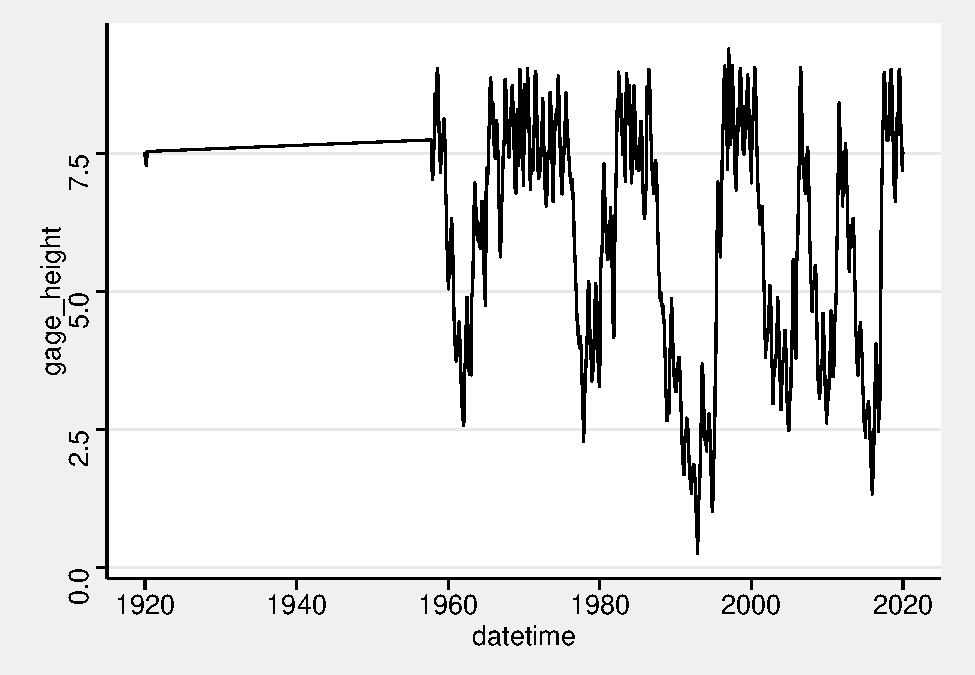
\includegraphics{data_exploration_files/figure-latex/unnamed-chunk-4-1.pdf}

\begin{Shaded}
\begin{Highlighting}[]
\KeywordTok{ggplot}\NormalTok{(USGS_gage_height) }\OperatorTok{+}
\StringTok{  }\KeywordTok{geom_point}\NormalTok{(}\KeywordTok{aes}\NormalTok{(}\DataTypeTok{x =}\NormalTok{ datetime, }\DataTypeTok{y =}\NormalTok{ gage_height))}
\end{Highlighting}
\end{Shaded}

\begin{verbatim}
## Warning: Removed 3 rows containing missing values (geom_point).
\end{verbatim}

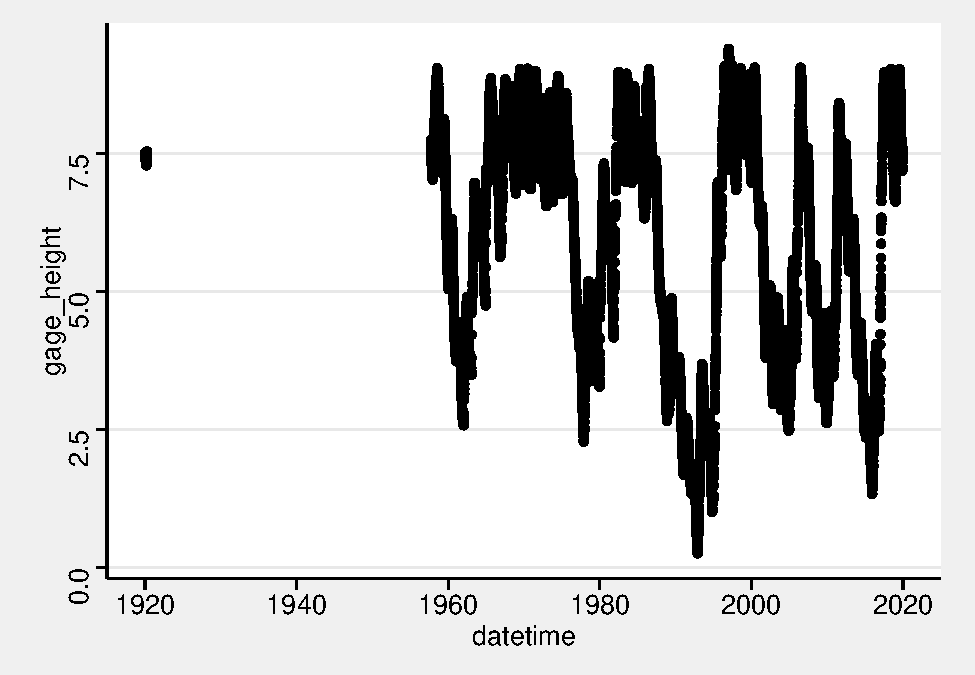
\includegraphics{data_exploration_files/figure-latex/unnamed-chunk-4-2.pdf}

\begin{Shaded}
\begin{Highlighting}[]
\CommentTok{#explore NOAA data}
\KeywordTok{ggplot}\NormalTok{(NOAA_climate, }\KeywordTok{aes}\NormalTok{(}\DataTypeTok{x =}\NormalTok{ DATE, }\DataTypeTok{y =}\NormalTok{ PRCP)) }\OperatorTok{+}
\StringTok{  }\KeywordTok{geom_line}\NormalTok{()}
\end{Highlighting}
\end{Shaded}

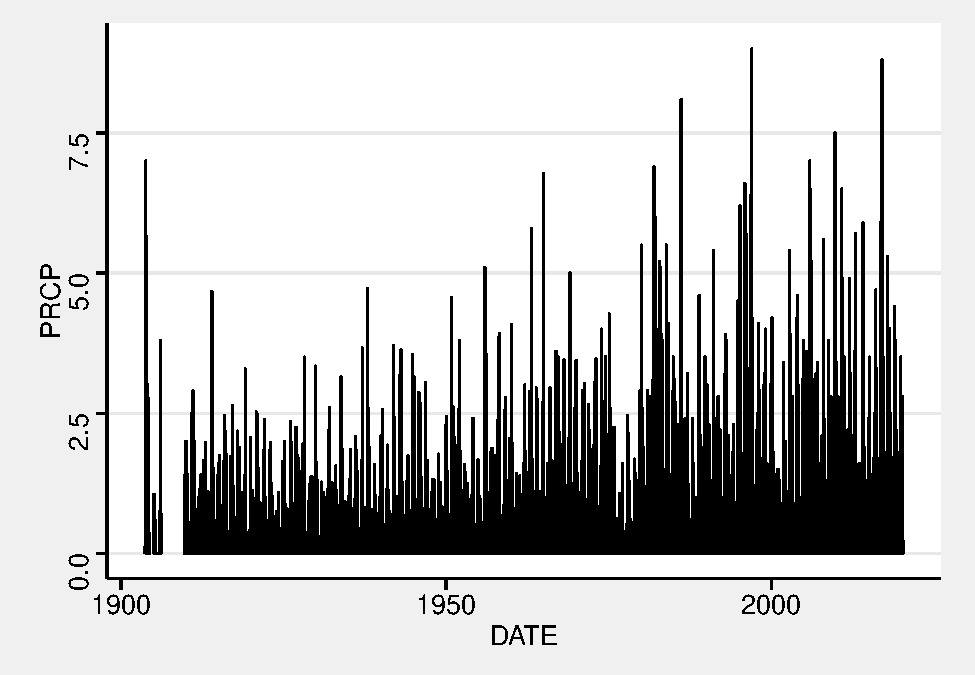
\includegraphics{data_exploration_files/figure-latex/unnamed-chunk-5-1.pdf}

\begin{Shaded}
\begin{Highlighting}[]
\KeywordTok{ggplot}\NormalTok{(NOAA_climate) }\OperatorTok{+}
\StringTok{  }\KeywordTok{geom_histogram}\NormalTok{(}\KeywordTok{aes}\NormalTok{(}\DataTypeTok{x =}\NormalTok{ PRCP), }\DataTypeTok{bins =} \DecValTok{20}\NormalTok{) }\OperatorTok{+}
\StringTok{  }\KeywordTok{xlim}\NormalTok{(}\DecValTok{0}\NormalTok{,}\DecValTok{5}\NormalTok{) }\OperatorTok{+}
\StringTok{  }\KeywordTok{ylim}\NormalTok{(}\DecValTok{0}\NormalTok{,}\DecValTok{8000}\NormalTok{)}
\end{Highlighting}
\end{Shaded}

\begin{verbatim}
## Warning: Removed 637 rows containing non-finite values (stat_bin).
\end{verbatim}

\begin{verbatim}
## Warning: Removed 2 rows containing missing values (geom_bar).
\end{verbatim}

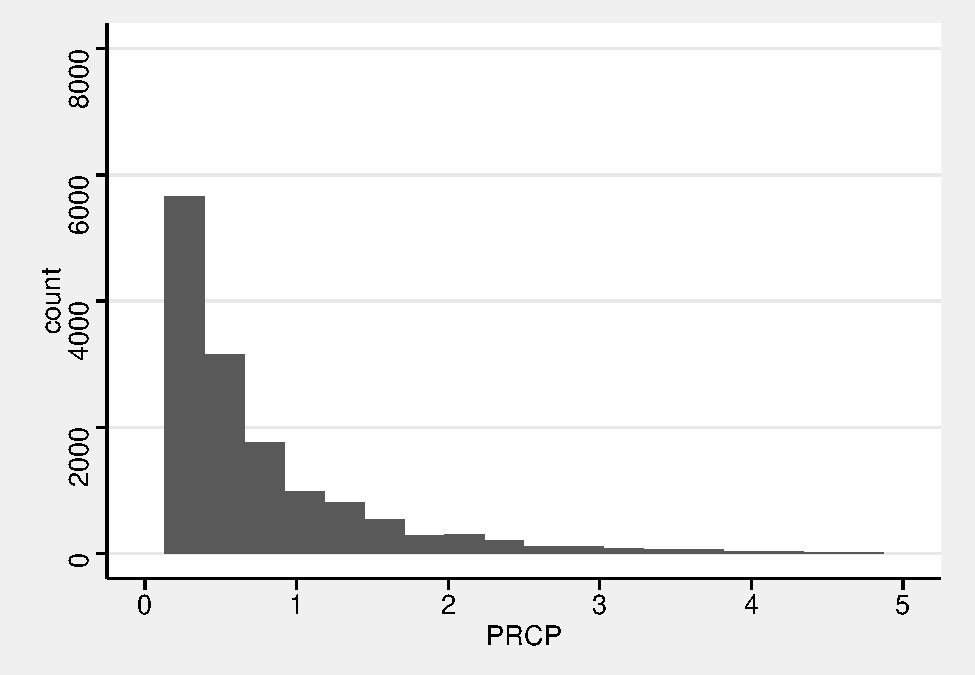
\includegraphics{data_exploration_files/figure-latex/unnamed-chunk-5-2.pdf}

\begin{Shaded}
\begin{Highlighting}[]
\KeywordTok{ggplot}\NormalTok{(NOAA_climate) }\OperatorTok{+}
\StringTok{  }\KeywordTok{geom_freqpoly}\NormalTok{(}\KeywordTok{aes}\NormalTok{(}\DataTypeTok{x =}\NormalTok{ PRCP), }\DataTypeTok{bins =} \DecValTok{50}\NormalTok{) }\OperatorTok{+}
\StringTok{  }\KeywordTok{geom_freqpoly}\NormalTok{(}\KeywordTok{aes}\NormalTok{(}\DataTypeTok{x =}\NormalTok{ TAVG), }\DataTypeTok{bins =} \DecValTok{50}\NormalTok{, }\DataTypeTok{color =} \StringTok{"blue"}\NormalTok{) }\OperatorTok{+}
\StringTok{  }\KeywordTok{geom_freqpoly}\NormalTok{(}\KeywordTok{aes}\NormalTok{(}\DataTypeTok{x =}\NormalTok{ SNOW), }\DataTypeTok{bins =} \DecValTok{50}\NormalTok{, }\DataTypeTok{lty =} \DecValTok{2}\NormalTok{)}
\end{Highlighting}
\end{Shaded}

\begin{verbatim}
## Warning: Removed 582 rows containing non-finite values (stat_bin).
\end{verbatim}

\begin{verbatim}
## Warning: Removed 57747 rows containing non-finite values (stat_bin).
\end{verbatim}

\begin{verbatim}
## Warning: Removed 46752 rows containing non-finite values (stat_bin).
\end{verbatim}

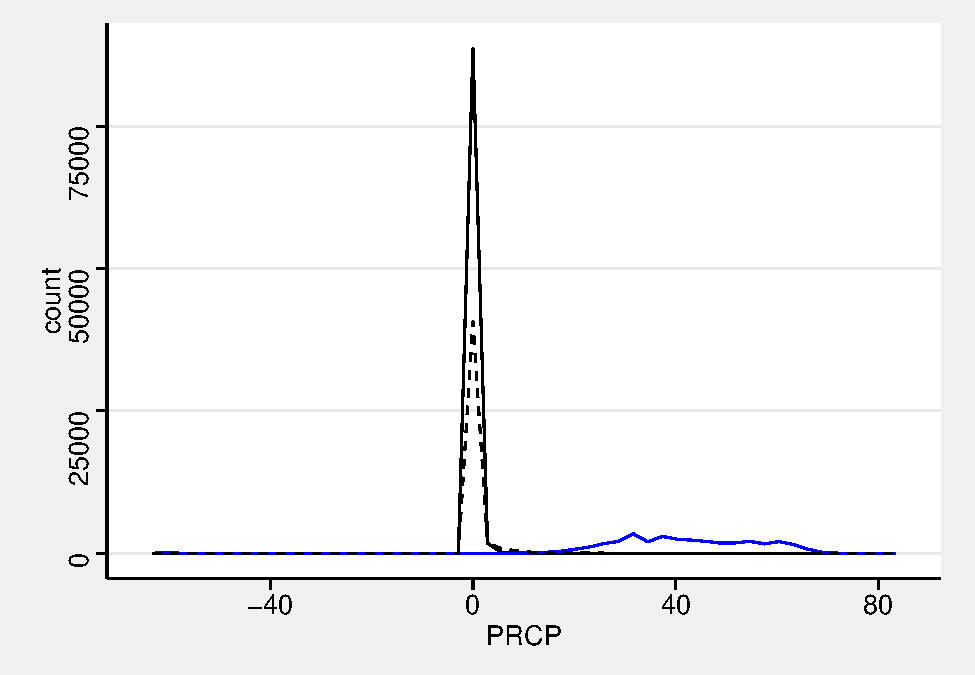
\includegraphics{data_exploration_files/figure-latex/unnamed-chunk-5-3.pdf}

\begin{Shaded}
\begin{Highlighting}[]
\KeywordTok{ggplot}\NormalTok{(NOAA_climate) }\OperatorTok{+}
\StringTok{  }\KeywordTok{geom_point}\NormalTok{(}\KeywordTok{aes}\NormalTok{(}\DataTypeTok{x =}\NormalTok{ PRCP, }\DataTypeTok{y =}\NormalTok{ TAVG))}
\end{Highlighting}
\end{Shaded}

\begin{verbatim}
## Warning: Removed 57749 rows containing missing values (geom_point).
\end{verbatim}

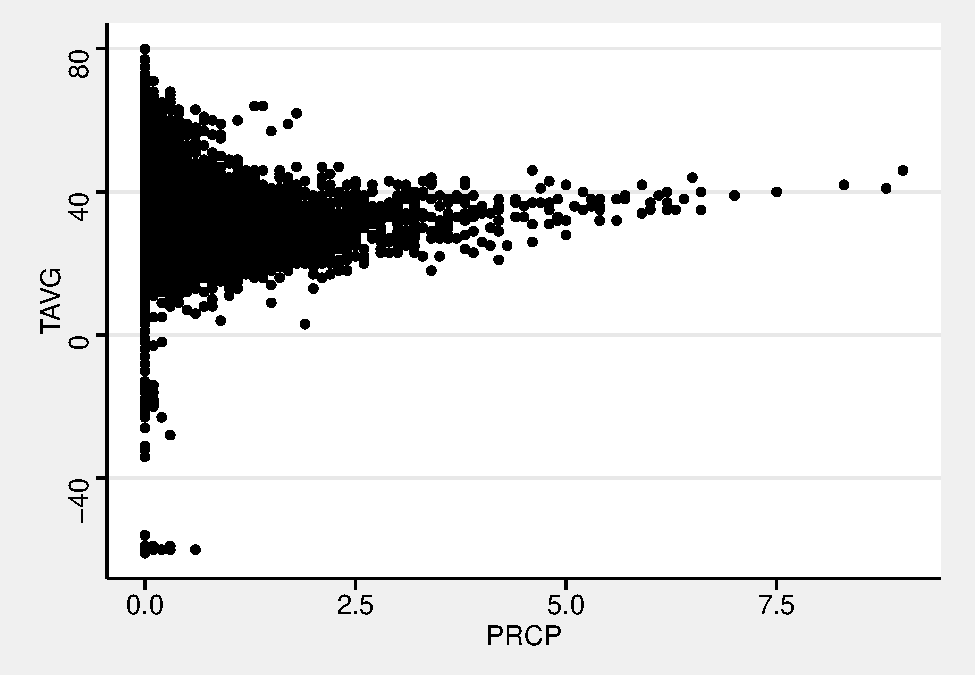
\includegraphics{data_exploration_files/figure-latex/unnamed-chunk-5-4.pdf}

\begin{Shaded}
\begin{Highlighting}[]
\KeywordTok{summary}\NormalTok{(NOAA_climate}\OperatorTok{$}\NormalTok{PRCP) }\CommentTok{#582 NAs}
\end{Highlighting}
\end{Shaded}

\begin{verbatim}
##    Min. 1st Qu.  Median    Mean 3rd Qu.    Max.    NA's 
##  0.0000  0.0000  0.0000  0.1255  0.0000  9.0000     582
\end{verbatim}

\begin{Shaded}
\begin{Highlighting}[]
\KeywordTok{summary}\NormalTok{(NOAA_climate}\OperatorTok{$}\NormalTok{SNOW) }\CommentTok{#46752 NAs}
\end{Highlighting}
\end{Shaded}

\begin{verbatim}
##    Min. 1st Qu.  Median    Mean 3rd Qu.    Max.    NA's 
##    0.00    0.00    0.00    0.56    0.00   49.00   46752
\end{verbatim}

\begin{Shaded}
\begin{Highlighting}[]
\KeywordTok{summary}\NormalTok{(NOAA_climate}\OperatorTok{$}\NormalTok{TAVG) }\CommentTok{#57747 NAs}
\end{Highlighting}
\end{Shaded}

\begin{verbatim}
##    Min. 1st Qu.  Median    Mean 3rd Qu.    Max.    NA's 
##  -61.00   32.00   41.00   41.88   53.00   80.00   57747
\end{verbatim}

\begin{Shaded}
\begin{Highlighting}[]
\KeywordTok{summary}\NormalTok{(NOAA_climate}\OperatorTok{$}\NormalTok{TMAX) }\CommentTok{#10883 NAs}
\end{Highlighting}
\end{Shaded}

\begin{verbatim}
##    Min. 1st Qu.  Median    Mean 3rd Qu.    Max.    NA's 
##  -61.00   43.00   54.00   55.43   69.00  452.00   10883
\end{verbatim}

\begin{Shaded}
\begin{Highlighting}[]
\KeywordTok{summary}\NormalTok{(NOAA_climate}\OperatorTok{$}\NormalTok{SNWD) }\CommentTok{#34812 NAs}
\end{Highlighting}
\end{Shaded}

\begin{verbatim}
##    Min. 1st Qu.  Median    Mean 3rd Qu.    Max.    NA's 
##    0.00    0.00    0.00   14.62   20.00  269.00   34812
\end{verbatim}

\begin{Shaded}
\begin{Highlighting}[]
\KeywordTok{summary}\NormalTok{(NOAA_climate}\OperatorTok{$}\NormalTok{TMIN) }\CommentTok{#10882 NAs}
\end{Highlighting}
\end{Shaded}

\begin{verbatim}
##    Min. 1st Qu.  Median    Mean 3rd Qu.    Max.    NA's 
##  -61.00   24.00   31.00   30.96   39.00   99.00   10882
\end{verbatim}

\begin{Shaded}
\begin{Highlighting}[]
\KeywordTok{levels}\NormalTok{(NOAA_climate}\OperatorTok{$}\NormalTok{NAME)}
\end{Highlighting}
\end{Shaded}

\begin{verbatim}
## [1] "SQUAW VALLEY G.C., CA US"   "SQUAW VALLEY, CA US"       
## [3] "TAHOE CITY CROSS, CA US"    "TAHOE CITY, CA US"         
## [5] "WARD CREEK NUMBER 3, CA US"
\end{verbatim}

\begin{Shaded}
\begin{Highlighting}[]
\KeywordTok{summary}\NormalTok{(NOAA_climate}\OperatorTok{$}\NormalTok{NAME)}
\end{Highlighting}
\end{Shaded}

\begin{verbatim}
##   SQUAW VALLEY G.C., CA US        SQUAW VALLEY, CA US 
##                      14481                       6691 
##    TAHOE CITY CROSS, CA US          TAHOE CITY, CA US 
##                      14426                      40638 
## WARD CREEK NUMBER 3, CA US 
##                      14792
\end{verbatim}

DO SUMMARY STATS TABLE

\#USGS Data

\begin{longtable}[]{@{}ll@{}}
\toprule
Parameter & Summary\tabularnewline
\midrule
\endhead
Total Number of Samples & 22,734\tabularnewline
Start Date & 1957-10-01\tabularnewline
End Date & 2019-12-31\tabularnewline
Gage Height (ft) Mean & 5.86\tabularnewline
Gage Height (ft) Median & 6.32\tabularnewline
Gage Height (ft) Min & 0.26\tabularnewline
Gage Height (ft) Max & 9.40\tabularnewline
\bottomrule
\end{longtable}

\#NOAA Climate Data

\begin{Shaded}
\begin{Highlighting}[]
\NormalTok{NOAA_summary <-}\StringTok{ }\KeywordTok{summary}\NormalTok{(NOAA_climate)}

\KeywordTok{kable}\NormalTok{(NOAA_summary, }\DataTypeTok{caption =} \StringTok{"Summary Table of NOAA Climate Raw Data"}\NormalTok{) }
\end{Highlighting}
\end{Shaded}

\begin{longtable}[]{@{}lcccccccccccc@{}}
\caption{Summary Table of NOAA Climate Raw Data}\tabularnewline
\toprule
& STATION & NAME & LATITUDE & LONGITUDE & ELEVATION & DATE & PRCP & SNOW
& SNWD & TAVG & TMAX & TMIN\tabularnewline
\midrule
\endfirsthead
\toprule
& STATION & NAME & LATITUDE & LONGITUDE & ELEVATION & DATE & PRCP & SNOW
& SNWD & TAVG & TMAX & TMIN\tabularnewline
\midrule
\endhead
& USC00048474: 6691 & SQUAW VALLEY G.C., CA US :14481 & Min. :39.14 &
Min. :-120.3 & Min. :1899 & Min. :1903-09-13 & Min. :0.0000 & Min. :
0.00 & Min. : 0.00 & Min. :-61.00 & Min. :-61.00 & Min.
:-61.00\tabularnewline
& USC00048758:40638 & SQUAW VALLEY, CA US : 6691 & 1st Qu.:39.17 & 1st
Qu.:-120.2 & 1st Qu.:1899 & 1st Qu.:1964-04-03 & 1st Qu.:0.0000 & 1st
Qu.: 0.00 & 1st Qu.: 0.00 & 1st Qu.: 32.00 & 1st Qu.: 43.00 & 1st Qu.:
24.00\tabularnewline
& USS0020K25S:14792 & TAHOE CITY CROSS, CA US :14426 & Median :39.17 &
Median :-120.2 & Median :1903 & Median :1989-01-31 & Median :0.0000 &
Median : 0.00 & Median : 0.00 & Median : 41.00 & Median : 54.00 & Median
: 31.00\tabularnewline
& USS0020K27S:14426 & TAHOE CITY, CA US :40638 & Mean :39.17 & Mean
:-120.2 & Mean :2035 & Mean :1981-10-12 & Mean :0.1255 & Mean : 0.56 &
Mean : 14.62 & Mean : 41.88 & Mean : 55.43 & Mean : 30.96\tabularnewline
& USS0020K30S:14481 & WARD CREEK NUMBER 3, CA US:14792 & 3rd Qu.:39.17 &
3rd Qu.:-120.1 & 3rd Qu.:2072 & 3rd Qu.:2004-08-29 & 3rd Qu.:0.0000 &
3rd Qu.: 0.00 & 3rd Qu.: 20.00 & 3rd Qu.: 53.00 & 3rd Qu.: 69.00 & 3rd
Qu.: 39.00\tabularnewline
& NA & NA & Max. :39.20 & Max. :-120.1 & Max. :2447 & Max. :2020-03-30 &
Max. :9.0000 & Max. :49.00 & Max. :269.00 & Max. : 80.00 & Max. :452.00
& Max. : 99.00\tabularnewline
& NA & NA & NA & NA & NA & NA & NA's :582 & NA's :46752 & NA's :34812 &
NA's :57747 & NA's :10883 & NA's :10882\tabularnewline
\bottomrule
\end{longtable}


\end{document}
